%-*- coding:UTF-8 -*-
%semiconductor.tex
%高温半导体材料调研
%编译环境xelatex->bibtex->xelatex->xelatex
\documentclass[UTF8, twocolumn]{ctexart}
\usepackage{graphicx}           %图表环境
%\usepackage{amsmath}            %公式环境
\usepackage{geometry}
\geometry{a4paper,left=2cm,right=2cm,top=2cm,bottom=2cm}
\usepackage[format=hang,font=small,textfont=it]{caption}
\CTEXsetup[format={\Large\bfseries}]{section}  %标题居左
\usepackage{abstract}
\renewcommand{\abstractname}{}
\usepackage{stfloats}
\usepackage{cite}
\usepackage{fancyhdr}
\renewcommand{\headrulewidth}{0.4pt}
\usepackage[colorlinks,linkcolor=black,citecolor=black]{hyperref}       %超链接


\title{\fangsong 高温超导体材料发展简述}
%\author{\kaishu 王展鹏}
\date{}

\bibliographystyle{unsrt}           %样式同plain,只是按照引用的先后排序
\pagestyle{fancy}

\begin{document}

\begin{titlepage}
    \heiti
    \vspace*{64pt}
    \begin{center}
        
        \begin{figure}
            \centering
            
\includegraphics[width=1.0\textwidth]{image/1.jpg} %1.jpg是图片文件的相对路径
            \label{img} %此处的label相当于一个图片的专属标志,目的是方便上下文的引用
        \end{figure}

        \fontsize{40pt}{0}{\kaishu  半导体材料课程报告}\\
        \vspace*{48pt}
    
        \LARGE 题目\ \ \underline{\makebox[200pt]{高温超导体材料发展简述}}\\
        \LARGE 作者\ \ \underline{\makebox[200pt]{王展鹏}}\\
        \LARGE 学号\ \ \underline{\makebox[200pt]{061710418}}\\
        \LARGE 学院\ \ \underline{\makebox[200pt]{材料科学与技术学院}}\\
        \LARGE 联系方式\ \ \underline{\makebox[200pt]{wwzzhhpp@nuaa.edu.cn}}\\
        \LARGE 指导老师\ \ \underline{\makebox[200pt]{李斌斌}}
        \vspace*{120pt}

        \LARGE 时间 \ \ \makebox[200pt]{2020 年 5 月}

    \end{center}
\end{titlepage}

\twocolumn[
\maketitle
\thispagestyle{fancy}

\begin{onecolabstract}
    \zihao{-4}\kaishu\noindent{摘要} 自从 1911 年超导现象被发现以来,为了能够将超导体用于生活的方方面面,无数科学家潜心研究,致力于提升超导体的临界温度、降低生产成本。本文简单介绍了超导材料和高温超导材料的发展历程,引用了国内外高温超导材料的发展情况,重点叙述了我国高温超导体在三个领域的应用。最后,高温超导作为战略高技术具有非常大的潜力,位列我国重大科技成果首位。

\end{onecolabstract}
]

\section{引言}

    超导体(Superconductor),指可以在特定温度以下,呈现电阻为零的导体。零电阻和完全抗磁性是超导体的两个重要特性。超导体电阻转变为零的温度,称为超导临界温度,据此超导材料可以分为低温超导体和高温超导体。虽然是高温超导,其实是相对于绝对零度而言,因此其温度可以远低于冰点摄氏$ 0 ^\circ C$。当温度很低时,超导体并没有太大的应用,科学家一直在寻求提高超导材料的临界温度,称之为“高温超导体”。

    \begin{figure*}[hb]
        \centering
        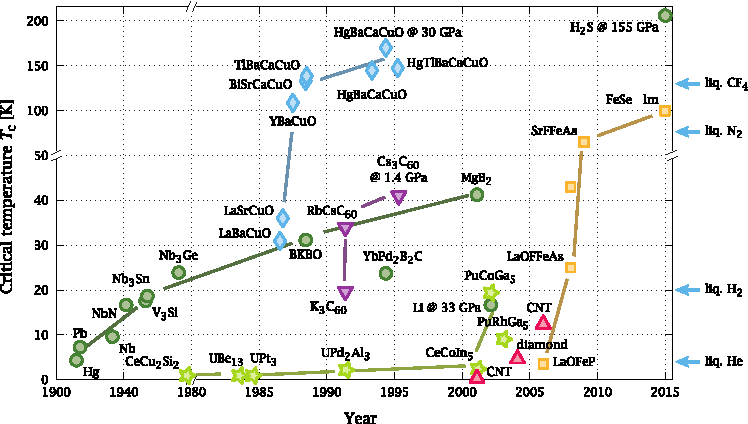
\includegraphics[scale=1.2]{image/Timeline_of_Superconductivity_from_1900_to_2015.pdf}
        \caption{自1911年首次发现以来,各种超导材料的超导临界温度概述}
        \label{fig:image1}
    \end{figure*}

    \subsection{超导体演化历史}
    1911年,荷兰科学家海克·卡末林·昂内斯用液氦冷却汞,发现当温度下降到绝对温标$4.2K$时水银的电阻完全消失,这种现象称为超导电性,将此温度称为临界温度。

    1933年,瓦尔特·迈斯纳和罗伯特·奥克森菲尔德两位科学家发现,如果把超导体放在磁场中冷却,则在材料电阻消失的同时,磁感应线将从超导体中排出,不能通过超导体,这种现象称为抗磁性。经过科学家的努力,磁电障碍已被跨越,下一个难关是突破温度障碍,寻求高温超导材料。

    2015年,德国普朗克研究所的 V.Ksenofontov 和 S.I.Shylin 研究组创下了新的超导温度记录:$203K$。其物质为硫化氢。

    图\ref{fig:image1}即为已发现的各种超导材料的超导临界温度及压力概述\cite{Ray2016}。

    \subsection{高温超导体简介}

    高温超导体(High-temperature superconductors)是超导物质中的一种族类,具有一般的结构特征以及相对上适度间隔的铜氧化物平面。它们也被称作铜氧化物超导体。此族类中一些化合物中,超导性出现的临界温度是已知超导体中最高的。不同铜氧化物在常态(以及超导态)性质之间具有共同的特征;这些性质中,许多无法以金属的传统理论来解释。

    \begin{figure*}[ht]
        \centering
        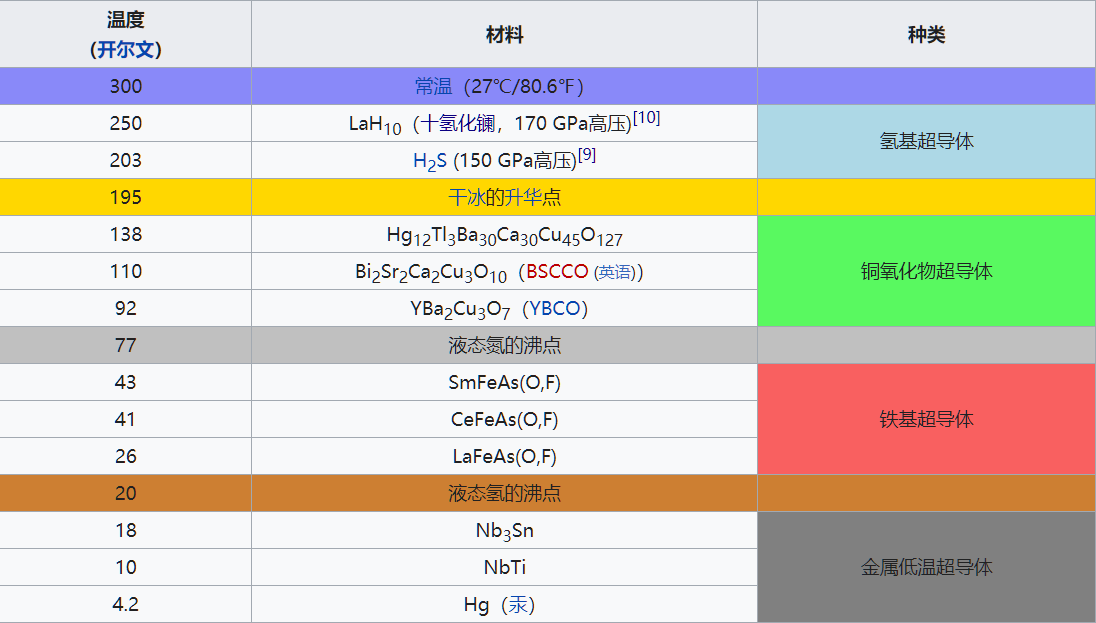
\includegraphics[scale=0.7]{image/超导材料.png}
        \caption{超导材料一览}
        \label{fig:image2}
    \end{figure*}

    如图\ref{fig:image2},当温度大于$77K$,超导材料被称为突破液氮的“温度壁垒”的材料。高温超导铜氧化物超导体等都是现在高温超导材料研究的热门材料。如钇钡铜氧化物$(YBCO)$,是化学式为$YBa_2 Cu_3 O_7$的化合物。它是著名的高温超导体,属于第二类超导体,并且是第一个制得转变温度在液氮沸点以上的材料。
    
    此外还有铁基超导体的发现。铁基超导体是指化合物中含有铁,在低温时具有超导现象,且铁扮演形成超导的主体的材料。引起许多科学家的兴趣的重要原因之一在于铁基超导体的结构与高温超导的铜氧平面类似,超导性发生在铁基平面上,属于二维的超导材料。因此尽管铁基超导体的临界温度只有数十$K$,研究铁基超导体可能有助于了解高温超导的机制。\cite{takahashi2008superconductivity}

\section{高温超导发展简史}

    铜氧化物超导体在实验上是由卡尔·米勒及约翰内斯·贝德诺尔茨首度发现。

    1987年,来自台湾的美国物理学家吴茂昆和朱经武在钇钡铜氧系材料上把临界温度提高到了$90K$以上。以吴茂昆为第一作者的论文\cite{PhysRevLett.58.908}发表以来已获期刊引用论文五千多次,史上第一次超越液态氮沸点“温度壁垒”将超导温度从$30K$提升到$90K$,被称为超导体领域30年来最重要的先驱之一。

    2001 年初发现的二硼化镁超导体\cite{nagamatsu2001superconductivity}临界温度可以达到 $39K$,其创造了金属间化合物超导材料临界温度的新纪录。转变温度较高,原料成本低廉,加工工艺简单等优点得到了广泛关注。其在$1-2T$磁场以及$10-20K$制冷机工作温度下的核磁共振成像系统中的超导应用上有着明显的技术和成本优势。

    2008 年日本学者 Hosono 发现铁基超导体材料\cite{kamihara2008iron},是继铜氧化合物超导体之后的第二个高温超导体。2014 年制备的铁基带材传输电流$J_c$在$4.2K/14T$下,已经达到了$100000A/cm^2$,标志着铁基超导材料已迈入实用化门槛。

    2015年,物理学者发现,硫化氢在极度高压的环境下(至少150$GPa$,也就是约150万标准大气压),约于温度203$K$时会发生超导相变\cite{drozdov2015conventional}。

    2018年,德国化学家发现十氢化镧有超导性出现,是目前已知最高温度的超导体。

    十氢化镧是镧和氢形成的氢化物之一,化学式为$LaH_{10}$,是一种多氢化物或超氢化物,有望用作高温超导体。它的超导转变温度$T_c$为约$250 K$,$(150 GPa)$,是2019年记录新高。其合成需要约160 $GPa$以上的压力。在1,000$ K$能够制得立方晶系的晶体,在室温得到的是六方晶系的晶体\cite{drozdov2019superconductivity}。

\section{国内外高温超导材料发展}
    
    \subsection{我国高温超导体发展情况}

    自从 1911 年超导现象被发现以来,经历了以$NbTi,Nb_3 Sn$等为代表的低温超导材料,以$Bi-Sr-Ca-Cu-O$为代表的第一代高温超导材料,以$Re-Ba-Cu-O$为代表的第二代高温超导材料,以及后期发现的$MgB_2$、铁基超导材料\cite{金之俭2018二代高温超导材料的应用技术与发展综述}。近 20 年来第二代高温超导材料研究成为了国内外超导研究的热点。我国已初步实现了第二代材料的动态制备\cite{杨天信2008我国高温超导技术研究现状}。

    自 1986 年发现高临界温度氧化物材料,开始了高临界温度超导电性研究的世界范围的热潮。我国超导体研究院积极开展 YBCO 高温超导块材的研究。在“九五”结束,北京金属研究总院已经基本建造了设备配套的研究基地,包括制粉、成材、测试等工序,研制的块材达到世界先进水平\cite{林良真2005我国超导技术研究进展及展望}。

    \subsection{国外高温超导体发展情况}

    早在 1987 年美国成立了非盈利公司超导体商业应用联合会,致力于超导技术产品商业化。2003 年 7 月美国公布《“Grid 2030" A National Vision for Electricity's Second 100 Years》\cite{doe2003grid}。报告中把高温超导技术列为美国电力网络未来 30 年发展的关键技术。该报告制定了未来 30 年的发展目标:在 2010 年前验证超导技术主干输电网络的可行性,实现 10 英里多相超导电缆应用;2020 年前实现 HTS 发电机、变压器等方面取得重要进展,实现长距离传到;2030 年前建成国家主干输电网络\cite{冯瑞华2008国外超导材料技术研究政策和方向}。2007 年,设计开发出了具有故障限流功能的钇系高温超导电缆;2009 年三芯电缆和终端安装在橡树岭国家实验室进行了故障限流测试和常规型实验,2014 年开始示范运行。

    1988 年日本成立了国际超导产业技术研究中心,致力于超导技术的调查研究和基础研究开发。 2005 年 3 月首次制定了国家层面的“战略技术路线图”,提出了在 2010 年大多数超导技术开始进入应用,在 2020 年达到普及。路线共分为四个部分:(1)能源电力:包括能源存储技术、输配电技术、发电技术;(2)工业交通:超导发动机、超导变压器技术;(3)医疗诊断:加速器技术等;(4)信息通讯:网络机器技术。并且将超导线材、块材、器材以及制冷与低温技术作为公共基础技术划分出来,在线材方面由 Nb 系列向低成本的 Bi 发展,块材则向氧化物系发展,低温制冷技术由小型制冷机向低成本、高功率制冷机发展。 

\section{我国高温超导体领域应用现状}

    \subsection{高温超导体在输电领域}

    我国能源资源和负荷的地理分布决定了我国电能输送具有划区域、远距离和大规模的特点,西南的水电、西北的火电、风电和太阳能发电将送至华北、华中、华南和南方从而形成大规模“西电东送”、“北电南送”电力流格局\cite{严陆光2014关于发展高温超导输电的建议}。为了提高能源、环境和经济等综合利用效率,从“十二五”起我国将大力发展特高压交流和直流输电。其中特高压交流定位于主网架建设和跨大区送电,直流定位于大型能源基地的远距离、大容量外送和跨网电源输送。

    电网的损耗主要源于输配电线路及变压器,其中输电线路损耗约占$1/3$,即大约为总发电功率的$2.5\%$左右。采用新的输电技术以提高电网的效率是十分重要和迫切的任务。

    目前,高温超导体的性能越来越接近实用化的水平,因此它以后再很多方面必将取代低温超导体,因此开展面向配电系统的高温超导体限流器的研究与开发工作非常有必要。同时还可以为以后从事其它超导电力设备和超导电力系统的研究和开发打下基础,并通过高温超导限流器的研究和试验运行使我国在高温超导的电力应用方面有重大技术突破并达到国际一流水平\cite{肖立业1999超导限流器}。

    \begin{figure*}[ht]
        \centering
        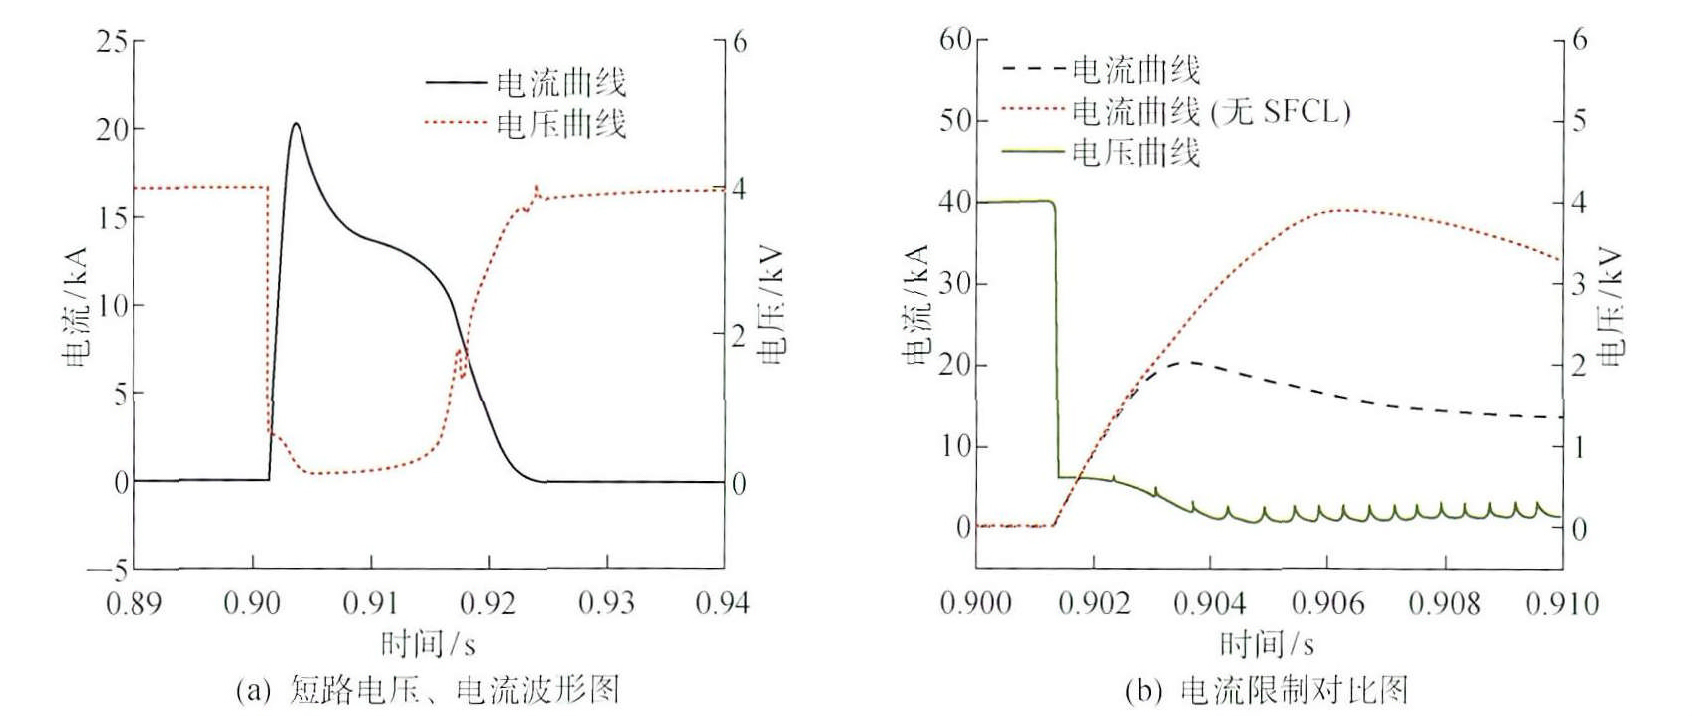
\includegraphics[scale=1]{image/直流限流器系统短路测试实验结果.jpg}
        \caption{直流限流器系统短路测试实验结果}
        \label{fig:image5}
    \end{figure*}

    上海交通大学在 2013 年完成了$4kV/2.5kA$高温超导直流限流器样机的研究工作,是当时国际上首次大容量直流限流器的尝试。试验结果如图 \ref{fig:image5} 所示,超导限流器接入直流系统后,系统短路电流由$39kA$下降至$20.4kA$,限流比达$47.71\%$,系统短路电流上升时间由$5ms$变为$2.4ms$,系统短路电流的分离点出现在短路发生后$1.5ms$,可认为超导限流器的响应时间为$1.5ms$,系统失超恢复时间$15s$。 2014 年课题组完成了$10kV/70A$高温超导电阻型交流限流器的挂网试验,为国内首次大容量高温超导电阻型限流器的尝试.接入超导限流器后,三相短路电流由$6.3kA$下降至$4.8kA$,短路电流下降了$23.8\%$,而系统电压由$4.2kV$提升至$5.1kV$,电压上升了$21.4\%$,超导限流器起到了明显的稳压效果\cite{金之俭2018二代高温超导材料的应用技术与发展综述}。

    \subsection{高温超导体在聚变领域应用}

    铜氧化物高温超导体主要有四大类:Bi(BiSrCuO,BSCCO),Y(YBaCuO,YBCO),TI(TIBaCaCuO),Hg(HgBaCaCuO),它们的各自临界温度都在$77K$,可以工作在液氮温区。\cite{孙林煜2012第二代高温超导体研究与在聚变领域应用前景}

    磁体线圈作为高温超导体的应用之一,是受控核聚变装置———托卡马克(Tokamak)的主要组成部分。在托卡马克装置中,由磁约束线圈电流和等离子体电流共同作用产生巨大的螺旋型磁场来约束真空室中的等离子体,使其与外界隔绝,然后通过欧姆加热线圈感应、中性束注入、离子回旋共振和电子回旋共振等方式将等离子体加热到上亿度的高温,实现核聚变反应并释放能量。

    初代托卡马克装置采用的是铜磁体线圈,其存在较大阻值损耗,而且在运行过程中产生大量的热,电流传输能力较低,磁场强度远远不能满足持续放电的要求。由于超导材料在临界温度下具有较高的临界电流密度和临界磁场强度,所以随着超导技术的发展,超导磁体得到了应用。然而低温超导磁体的临界温度太低,只能在复杂昂贵的液氦($4.2K$)系统中使用。高温超导材料的出现突破了温度壁垒,把超导应用的温度从液氦($4.2K$)温区提高到了液氮($77K$)温区,大幅度地节省了制冷费用。目前第一代$Bi$系高温超导线材的制备技术成熟,然而其临界电流密度和临界磁场强度较低,磁场稳定性较差等因素,使得$Bi$系高温超导应用受到了极大地限制。第二代高温超导材料的制备工艺较为复杂,目前还未得到大规模的生产。但是其具有较高的临界电流密度和临界磁场强度,较好的磁场稳定性,较低的交流损耗等优势,使得第二代高温超导材料具有很大的应用前景。随着高温超导技术的不断发展,有望在未来的示范堆中得到应用。同时利用高温超导材料作为超导的电流引线,会大大减少磁体系统的热负荷,降低制冷费用,而且高温超导电流引线不需要补充液氮,仅通过热机即可实现低温\cite{孙林煜2012第二代高温超导体研究与在聚变领域应用前景}。

    \subsection{高温超导体磁悬浮技术研究}
    高温超导磁悬浮利用高温超导体在混合态中的磁通钉扎特性以及抗磁性来实现稳定悬浮。这种自稳定悬浮无需外加能量输入,抗干扰能力强,相比于其它悬浮方式具有非常明显的优势。\cite{刘文旭2020高温超导磁悬浮技术研究论述}

    2000 年,我国引进德国磁悬浮 TR08 系列磁悬浮列车,建成上海浦东机场线,并于 2004 年正式投入商业运营\cite{1643050}。长沙磁浮快线工程于2014年5月16日正式开工,于2015年下半年建成,于12月26日开始试运行,并于2016年5月6日投入载客试运营。2019 年 5 月 23 日,我国时速 600 $km$,高速磁悬浮试验样车在青岛下线。

    2000 年 12 月,我国西南交通大学已经完成了世界上第一辆载人高温超导磁悬浮试验车系统。该课题于 2001 年 2 月 11 日通过了由国家“863”计划国家超导技术专家委员会首席专家甘子钊院士主持的验收。验收会议认为:此项成果“是长期努力的创造性成果,它开拓了在磁悬浮技术上实现创新跨越发展的可能性。”所用到的高温超导钇钡铜氧块材,我国已经具备了批量生产的能力,高温超导磁悬浮技术所需的特殊原材料钇和钕均属于我国富有的稀土元素。与现在我国已从德国引进的常导磁悬浮列车相比,不仅具有其不可及的一系列优点,而且拥有我国自己的全部知识产。\cite{沈志云2012在我国建设世界上第一条高温超导磁悬浮列车试运行线的建议}

    2006 年,西南交通大学王家素团队设计了一种高温超导磁悬浮系统。发射系统是由悬浮滑车、永磁体轨道和直线电机组成。车辆由车载HTS、磁浮装置和车体组成。该高温超导磁悬浮发射系统的永磁轨道长10.05 m、宽0.68 m。真空输送管(ETT) 中真空管的框架长11.2 m、宽1.0 m。真空管相对于水平方向的纵坡为$0\sim 30^\circ$,与水平方向的横坡为$15^\circ$。高温超导磁悬浮发射车长1.0$m$、宽1.0$m$。\cite{pan2011influence}

    \begin{figure}[ht]
        \centering
        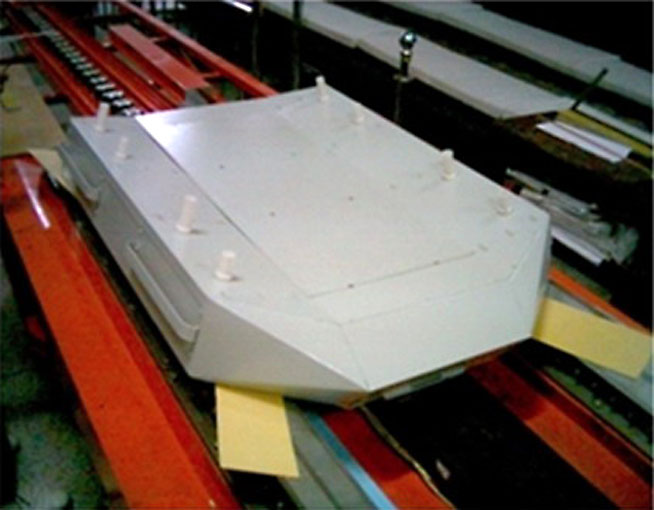
\includegraphics[scale=0.8]{image/pan2010.jpg}
        \caption{HTS磁悬浮发射平台的悬浮体}
        \label{fig:image3}
    \end{figure}

\section{我们的工作}

    中国科学院系统梳理了改革开放 40 周年来中科院广大广大科研人员取得的众多重大科技成果,以“三个面向”为线索,综合凝结归纳出 40 项具有代表性的标志性重大科技成果。40 项标志重大成果经学术委员会委员审核把关,通过网络向院属单位和社会进行了公示,已收录于《改革开放先锋 创新发展引擎——中国科学院改革开放四十年》\footnote{中国科学院改革开放四十年40项标志性重大科技成果. 中国科学院院刊, 2018, 33(12): 1282-1313}一书,现予以公布。
    
    其中高温超导体研究位于\href{http://www.bulletin.cas.cn/publish_article/2018/12/20181202.htm}{ 40 项重大科技成果}首位。中国科大和物理研究所在铁基超导体研究方面先后在国际上首次突破了麦克米兰极限温度\footnote{科学家麦克米兰根据获1972年诺贝尔奖的BCS理论计算,认为超导临界温度最高不大可能超过 40$K$ ,他的计算得到了国际学术界的普遍认同,40$K$ 也因此被称作“麦克米兰极限”。},确定铁基超导体为新一类高温超导体,并在物理性质研究方面取得重要成果,具有潜在应用价值,获得 2013 年国家自然科学一等奖。

    \begin{figure}[h]
        \centering
        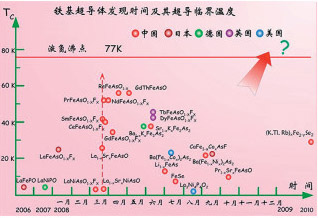
\includegraphics[scale=0.8]{image/铁基超导体.jpg}
        \caption{铁基超导体发现时间及其超导临界温度}
        \label{fig:image4}
    \end{figure}

\section{总结}

    氧化物高温超导材料将会是液氮温区下强电应用的主角,应用前景广泛。以YBCO图层导体为代表的第二代高温超导带材正处于产业化前夜,人们正在努力推动起向低成本、稳定化和规模化方向发展\cite{马衍伟2015实用化超导材料研究进展与展望}。

    超导技术作为 21 世纪的战略高技术,被世界各大国所重视,特别是实用化超导材料的研究与应用一直是国际最激烈也是最活跃的领域之一。

\kaishu
\addcontentsline{toc}{section}{参考文献}
\bibliography{main.bib}


\end{document}A